\section{méthodologie}
\subsection{Agile manifesto}

%\textbf{Manifesto for Agile Software Development }\\
%We are uncovering better ways of developing
%software by doing it and helping others do it.
%Through this work we have come to value:
\begin{enumerate}
    \item  Individuals and interactions over processes and tools
    \item Working software over comprehensive documentation
    \item Customer collaboration over contract negotiation
    \item Responding to change over following a plan 
\end{enumerate}

%That is, while there is value in the items on the right, we value the items on the left more. 

\subsection{Scrum/Agile}
\begin{wrapfigure}{r}{0.25\textwidth} 
    \centering
    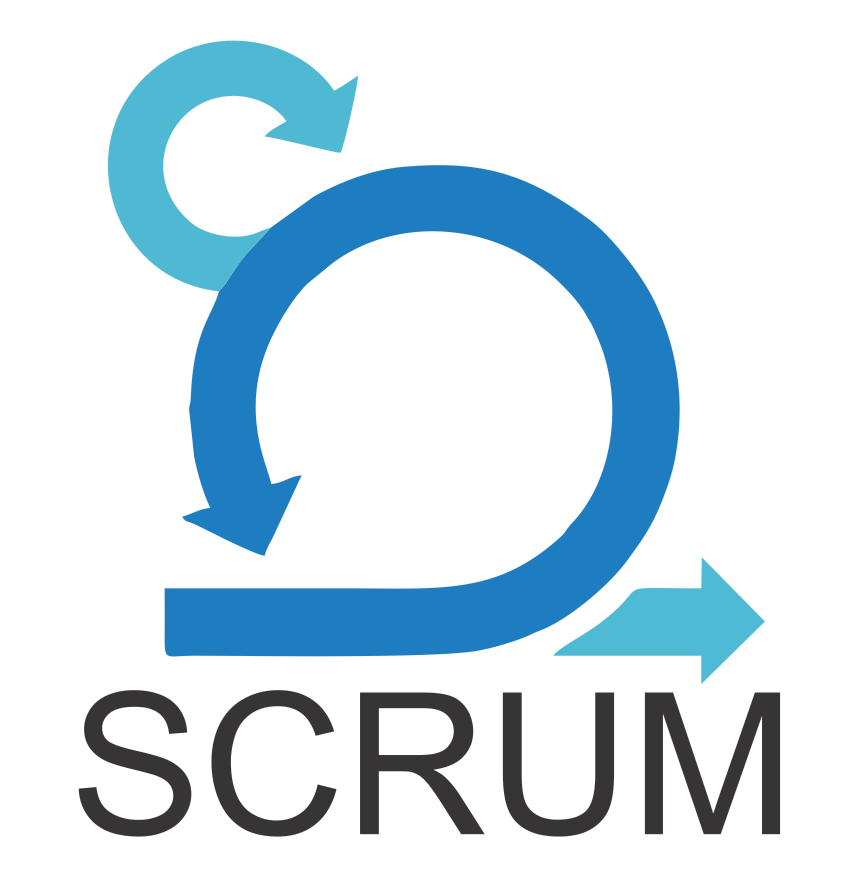
\includegraphics[width=0.25\textwidth]{scrum logo.png}
    \caption{logo de scrum Agile}
\end{wrapfigure}
Selon The Scrum GuideTM, Scrum est « un framework léger qui aide les personnes, les équipes et les organisations à générer de la valeur grâce à des solutions adaptatives à des problèmes complexes.1 » Scrum est le framework agile le plus largement utilisé et le plus populaire. Le terme agile décrit un ensemble spécifique de principes et de valeurs fondamentaux pour l'organisation et la gestion d'un travail complexe.
Bien qu'il ait ses racines dans le développement de logiciels, Scrum fait aujourd'hui référence à un cadre léger utilisé dans tous les secteurs pour fournir des produits et services complexes et innovants qui ravissent réellement les clients. C'est simple à comprendre, mais difficile à maîtriser.
\cite*{scrumalliance}

\section{téchnologies}

\subsection{Android}
\begin{wrapfigure}{r}{0.25\textwidth} 
    \centering
    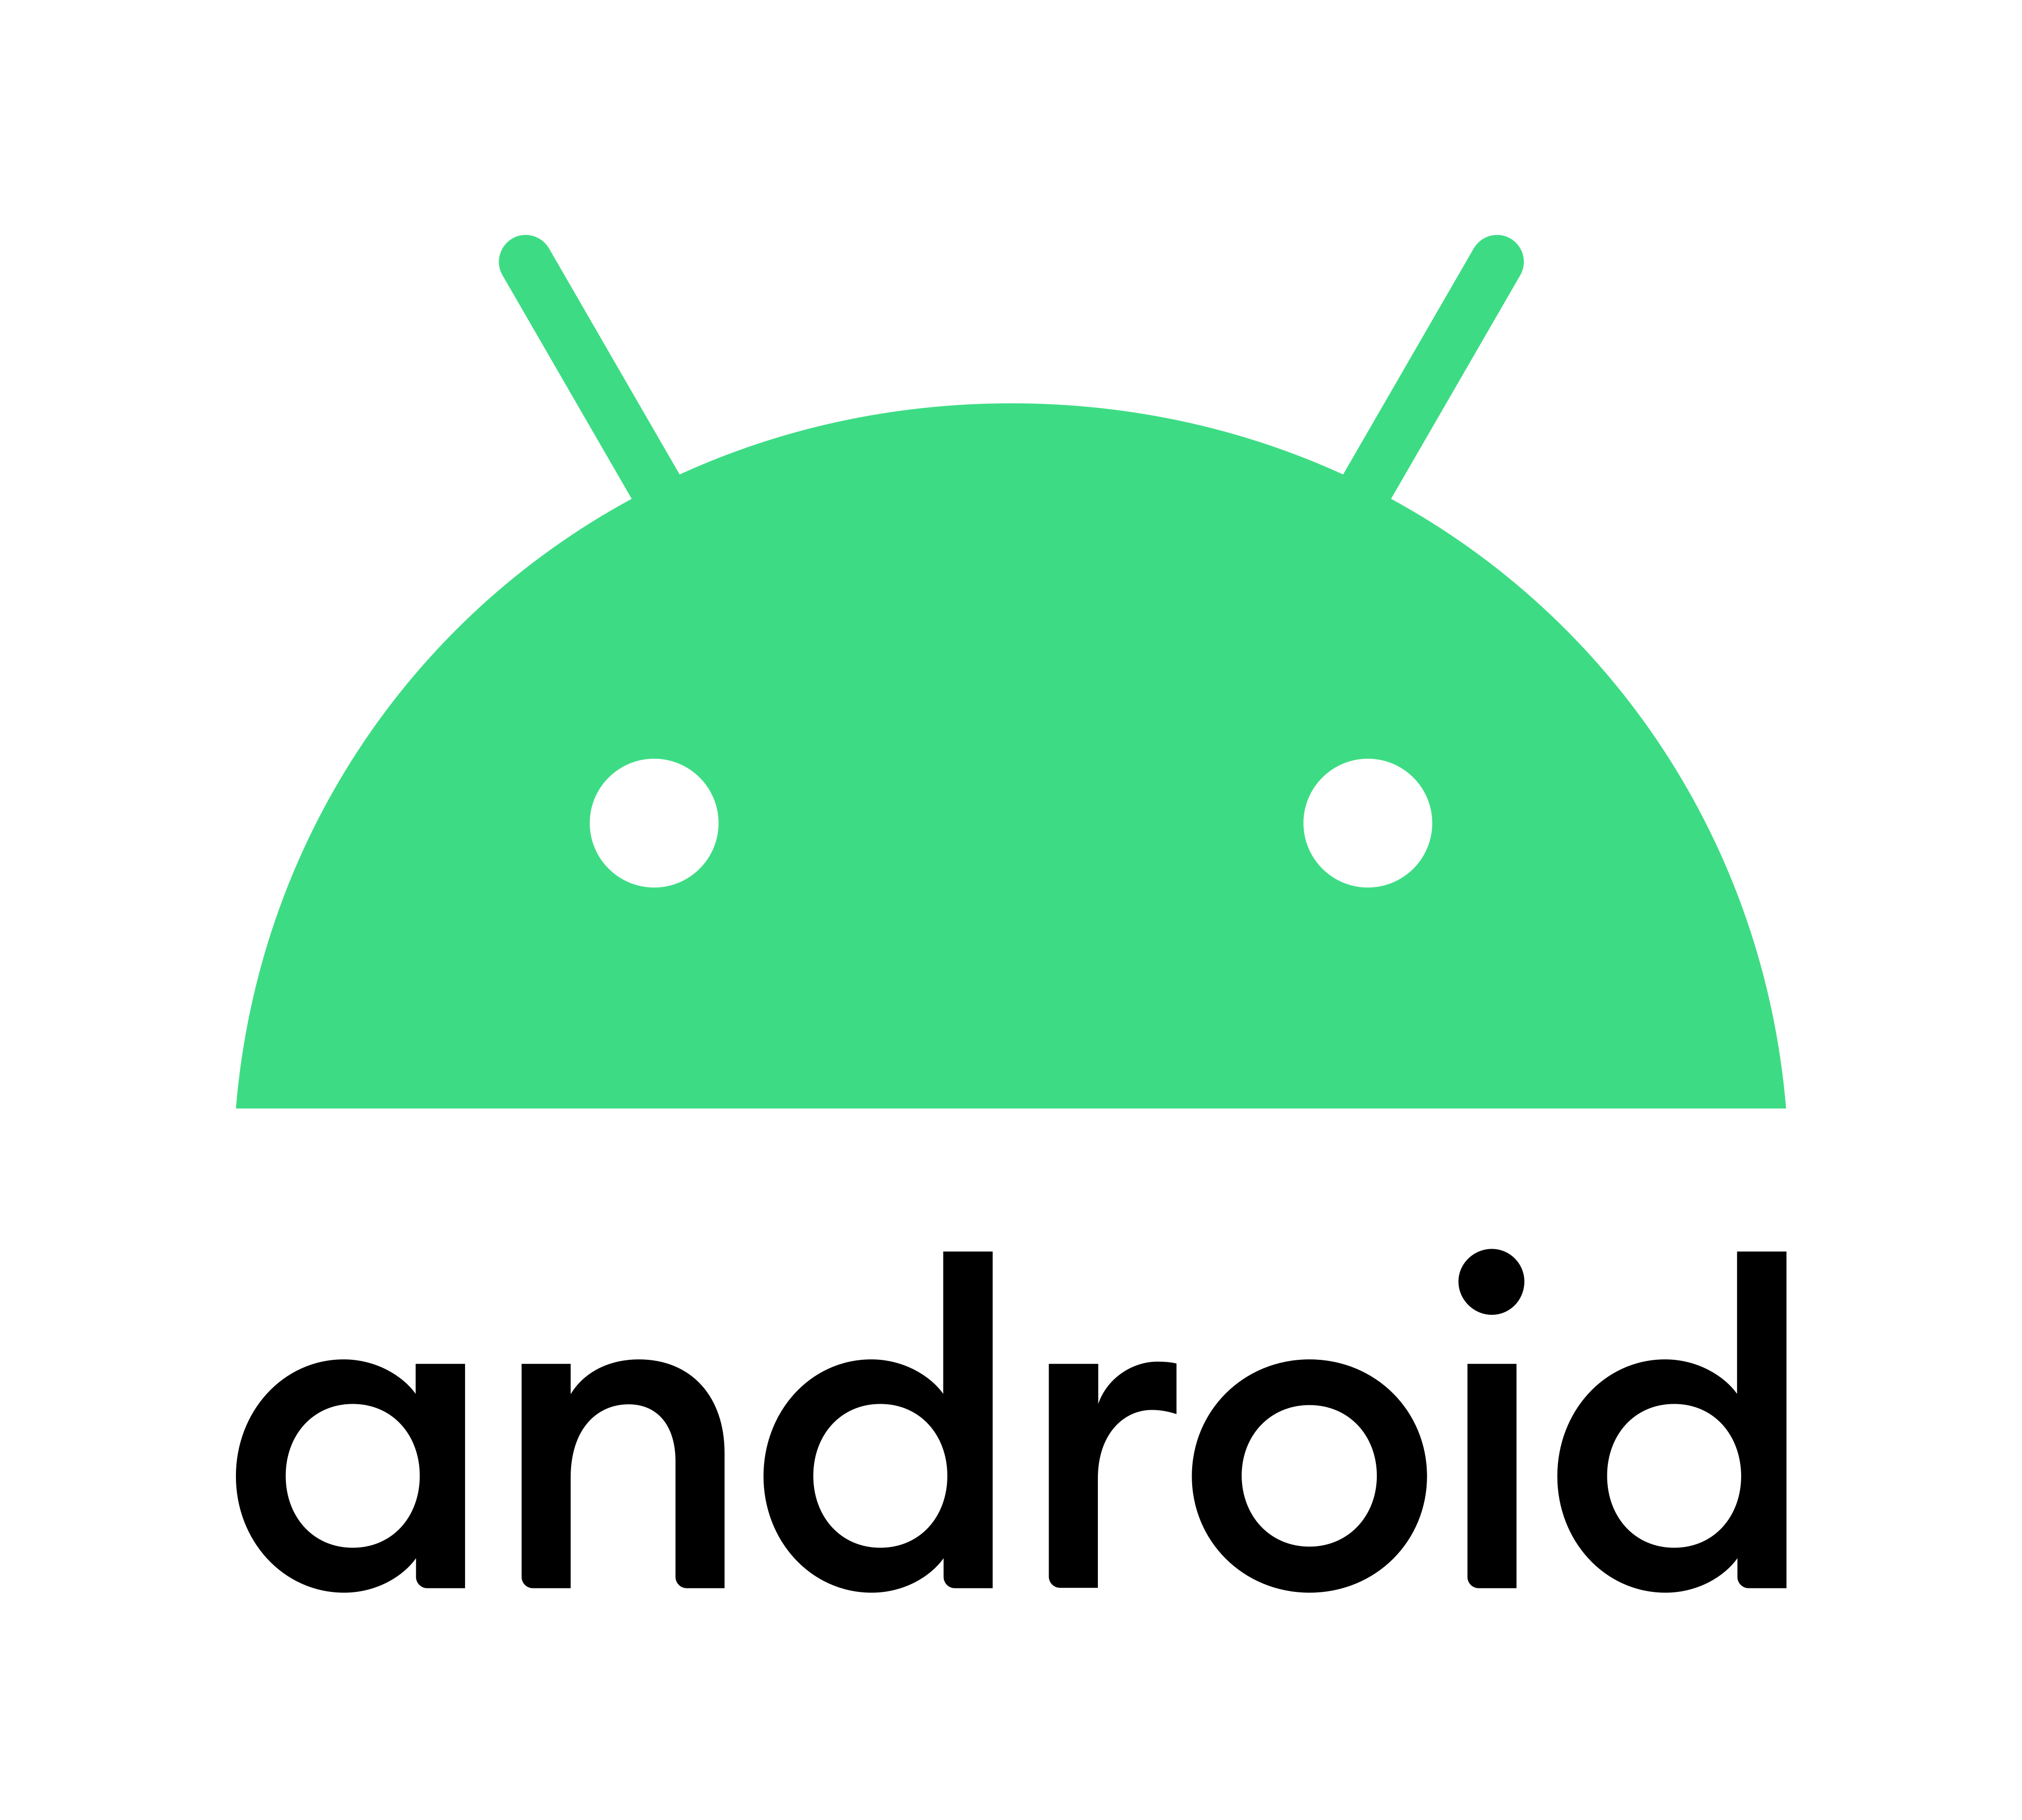
\includegraphics[width=0.25\textwidth]{android-logo.png}
    \caption{logo d'android}
\end{wrapfigure}
Android est un système d'exploitation mobile open source fondé sur le noyau Linux et développé par un consortium d'entreprises, le Open Handset Alliance, sponsorisé par Google. 
Android est défini comme étant une pile de logiciels, c'est-à-dire un ensemble de logiciels destinés à fournir une solution clé en main pour les appareils mobiles, smartphones et tablettes tactiles. Cette pile comporte un système d'exploitation (comprenant un noyau Linux), les applications clés telles que le navigateur web, le téléphone et le carnet d'adresses ainsi que des logiciels intermédiaires entre le système d'exploitation et les applications
\cite*{wiki:Android}

\subsection{Kotlin}
\begin{wrapfigure}{r}{0.25\textwidth} 
    \centering
    
\includegraphics[width=0.25\textwidth]{kotlin.png}
    \caption{logo de Kotlin}
\end{wrapfigure}
Kotlin est un langage de programmation orienté objet et fonctionnel, avec un typage statique qui permet de compiler pour la machine virtuelle Java, JavaScript, et vers plusieurs plateformes en natif (grâce à LLVM). Son développement provient principalement d'une équipe de programmeurs chez JetBrains basée à Saint-Pétersbourg en Russie (son nom vient de l'île de Kotline, près de St. Pétersbourg).
Google annonce pendant la conférence Google I/O 2017 que Kotlin devient le second langage de programmation officiellement pris en charge par Android après Java. Le 8 mai 2019, toujours lors de la conférence Google I/O, Kotlin devient officiellement le langage de programmation voulu et recommandé par le géant américain Google pour le développement des applications Android.
Pivotal Software annonce le 4 janvier 2017 le support officiel de Kotlin sur la cinquième version du Framework Spring. 
\cite*{wiki:Kotlin}
\subsection{les bonnes pratiques}
TO BE IMPLEMENTED
\subsection{GitHub}
TO BE IMPLEMENTED
\subsection{Android JetPack Compose}
TO BE IMPLEMENTED
\subsection{Gradle}
TO BE IMPLEMENTED
\subsection{Firebase}
TO BE IMPLEMENTED
\subsection{Firebase FireAuth}
TO BE IMPLEMENTED
\subsection{Firebase FireStore}
TO BE IMPLEMENTED
